\documentclass[12pt]{article}
\usepackage[margin=2.53cm]{geometry}
\usepackage[french]{babel}
\usepackage[utf8]{inputenc}
\usepackage[T1]{fontenc}
\setlength{\parindent}{0pt}
\setlength{\parskip}{1em}
\usepackage{hyperref}
\usepackage{graphicx}
\topskip0pt
\usepackage{xcolor}
\usepackage{enumitem}
\usepackage[printonlyused]{acronym}
\usepackage{multicol}
\usepackage{amsmath, amstext, amsfonts, amssymb}
\usepackage{tikz}
\usepackage{commath}
\usepackage{booktabs}
\usepackage{multirow}
\newlist{abbrv}{itemize}{1}
\setlist[abbrv,1]{label=,labelwidth=1in,align=parleft,itemsep=0.1\baselineskip,leftmargin=!}
\newcommand{\notation}[1]{\textcolor{blue}{{#1}}}

\newif\ifnotes
\makeatletter
\newcommand{\note}[1]{\@bsphack\ifnotes{#1}\fi\@esphack}
\makeatother
\newcommand{\nonotes}{\notesfalse}
\newcommand{\capitalLetter}[1]{\textsc{\MakeLowercase{#1}}}

%%%%%%%%%%%%%%%%%%%%% Section à remplir %%%%%%%%%%%%%%%%%%%%%
\newcommand{\titreDuCours}{\textit{titre du cours}}
\newcommand{\sigleCoursStage}{\textit{sigle}}
\newcommand{\session}{\textit{session}}

\newcommand{\titreEtudiant}{\textit{titre etudiant}}
\newcommand{\titreTravail}{\textit{titre travail}}
\newcommand{\nomOrganisation}{Université Laval}

\newcommand{\dateRemise}{\textit{date de remise}}
\newcommand{\prenomStagiaire}{\textit{prenom}}
\newcommand{\nomStagiaire}{\textit{nom}}
\newcommand{\idul}{\textit{idul}}

\newcommand{\prenomSuperviseur}{\textit{prenom personne remettre}}
\newcommand{\nomSuperviseur}{\textit{nom personne remettre}}
\newcommand{\titreSuperviseur}{\textit{titre personne remettre}}

\newcommand{\distTitreTravailEtNom}{4cm}
\newcommand{\distanceTypeRapportEtDestinataire}{5cm}
%%%%%%%%%%%%%%%%%%%%%%%%%%%%%%%%%%%%%%%%%%%%%%%%%%%%%%%%%%%%%

\begin{document}
	\thispagestyle{empty}
	\begin{minipage}[t]{8.1cm}
		\vspace{0pt}
		\begin{flushleft}
			\hspace{-1cm}
			
\includegraphics[width=5cm]{../img/UL-FSG-C-g-3lignes.png}
			\\
		\end{flushleft}
	\end{minipage}
	\begin{minipage}[t]{8.1cm}
		\begin{flushright}
			\hspace*{2cm} \\ \hspace*{1cm}\titreDuCours\\ \hspace*{1cm}\sigleCoursStage\\ \hspace*{1cm}\session\\
			\hspace*{1cm} Date de remise : {\dateRemise}\\
		\end{flushright}
	\end{minipage}

	\vspace{\distTitreTravailEtNom}
	\begin{center}
		\fontsize{14.4}{14.4}\large \textbf{Rapport de stage}\\
		\vspace{1cm}
		\large {\titreTravail} \\
		\vspace{0.2cm}
		{\nomOrganisation} \\
		\vspace{\distanceTypeRapportEtDestinataire}
		\fontsize{14.4}{14.4}\textbf{Destinataire}\\ \large \textit{ajouter le destinataire}
		- Direction de la Faculté des sciences et de génie \\
		\vspace{0,5cm}
		\large \prenomSuperviseur~\nomSuperviseur~- \titreSuperviseur \\
	\end{center}
	\vspace{3cm}

	\begin{minipage}[t]{6cm}
		\begin{flushleft}
			\textbf{\prenomStagiaire~\nomStagiaire}\\
		\end{flushleft}
	\end{minipage}
	\begin{minipage}[t]{10cm}
		\begin{flushright}
			\hspace*{1cm}\textbf{\idul} \\
		\end{flushright}
	\end{minipage}

	\newpage
	\pagenumbering{Roman}

	\newpage
	\tableofcontents

	\newpage
	\listoftables

	\newpage
	\listoffigures

	\newpage
	\addcontentsline{toc}{section}{\numberline{}Liste de symboles et abréviations}
\textbf{Liste de symboles et abréviations}

\bigskip

\begin{acronym}
	\acro{OMERO}{Open Microscopy Environment Remote Object} \acro{GRPM}{groupe de recherche en physique médicale}
	\acro{AD}{Active Directory} \acro{DNS}{Domain Name System} \acro{IP}{Internet Protocol}
	\acro{MJQ}{Ministère de la Justice}
\end{acronym}

\acresetall
	\break

	\newpage
	\pagenumbering{arabic}

	\section{Section 1}

\subsection{Sous-section 1}
ajouter les sections dans de nouveaux fichiers et sous-sections nécessaires dans le même
fichier correspondant avec l'ordre pour le premier chiffre

\subsection{Sous-section 2}

	\section{TUTORIEL POUR LA BIBLIOGRAPHIE}
	Ajoutez vos sources au document \textbf{references.bib}.

	\textbf{Citer une source} : \textbackslash cite\{SOURCE\} pour obtenir ceci :
	\cite{howard2020deep}.

	\textbf{Citer plusieurs sources} : \textbackslash cite\{SOURCE1, SOURCE2\} pour obtenir
	ceci : \cite{goodfellow2014generative, CycleGAN2017}.
	\section{TUTORIEL POUR LES FIGURES}

	\textbf{Citer une figure} : \textbackslash ref\{fig:NOM\}. Par exemple, voir la Figure~\ref{fig:gan}
	ou l'annexe \ref{appendix:fastbook}.

	Pour chaque figure, faire figurer un titre pertinent qui en explique le contenu. Pour que
	votre document reste agréable à travailler, mettre toutes vos images dans le dossier "img".

	\begin{figure}[!h]
		\begin{center}
			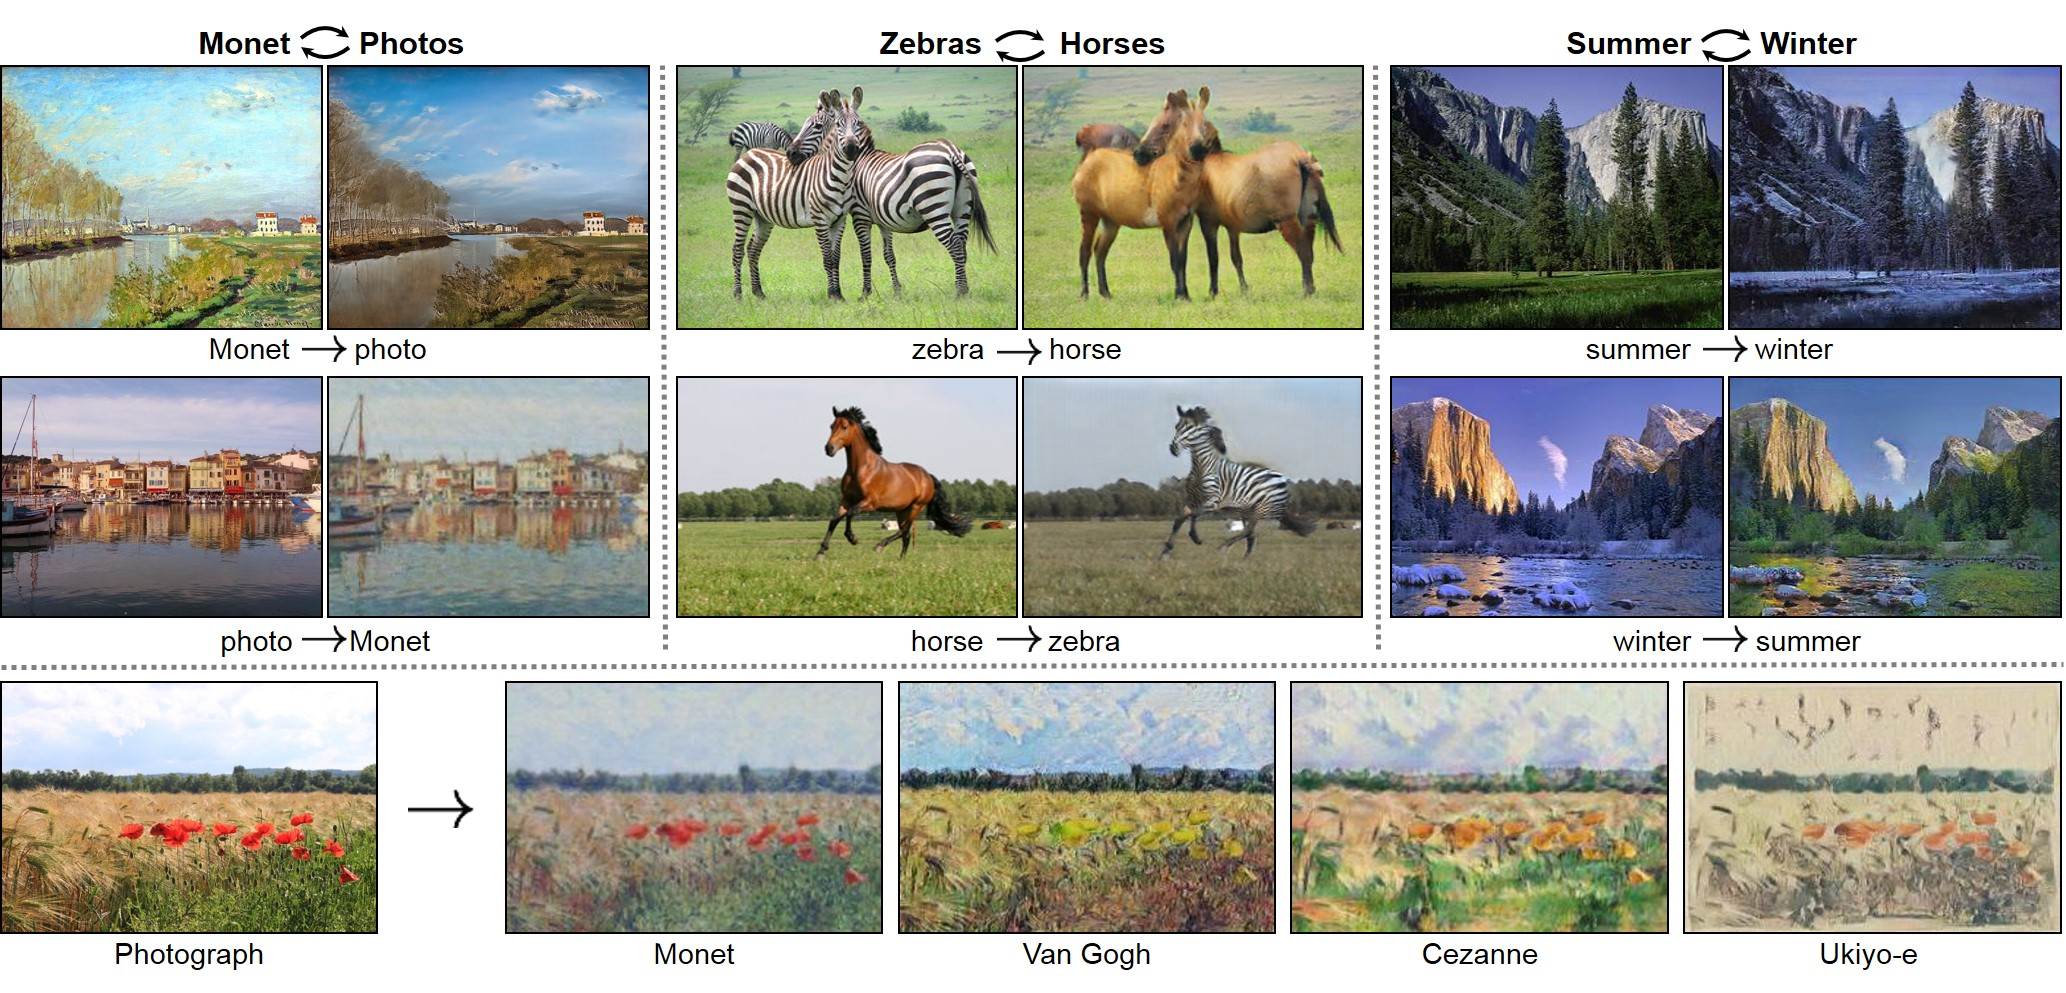
\includegraphics[scale=0.4]{../img/gan_img.jpg}
		\end{center}
		\caption{Figure dans le texte~\cite{CycleGAN2017}}
		\label{fig:gan}
	\end{figure}
	\newpage
	\appendix

	\section{TUTORIEL POUR L'ANNEXE \#1}
	\label{appendix:consigne}
	\begin{enumerate}
		\item Exemples d’informations pouvant figurer dans les annexes : photos, croquis, figures
			et schémas, tableaux de données, fiche de relevés, etc.

		\item S’il y lieu, les calculs doivent apparaître en annexe (une seule annexe pour tous
			les calculs du rapport). Il est important de donner clairement les hypothèses de calculs,
			de citer les références des formules employées et de donner les valeurs des
			diverses variables et les résultats des calculs.

		\item S’il y a lieu, inclure des annexes supplémentaires pour consigner les
			photocopies de catalogues sur des produits particuliers, la correspondance avec les
			clients ou fournisseurs, les tableaux de résultats, les formulaires divers, les
			plans de fabrication, résultats de simulation ou autres.

		\item Il faut désigner les annexes de façon à ce que l’on puisse identifier son contenu
			(ex. : Annexe B : Spécifications techniques). En pratique, on sépare les annexes
			par des onglets d’identification. Chaque page d’une annexe est numérotée (ex. : B1,
			B2, …) et on retrouve au début de chaque annexe une liste du contenu. Attention de
			ne pas multiplier les annexes à outrance.
	\end{enumerate}
	Chaque annexe est annoncée deux fois :
	\begin{enumerate}
		\item Dans la table des matières;

		\item Dans le corps du rapport, sous la forme d’un renvoi.
	\end{enumerate}

	Pour citer votre annexe dans le texte, il suffit d'utiliser la commande \ref{appendix:consigne}.
	De même pour \ref{appendix:fastbook}. La configuration de ce document permet d'inclure
	directement votre annexe dans la table des matières

	\section{TUTORIEL POUR L'ANNEXE \#2}
	\label{appendix:fastbook}
	\begin{center}
		
\includegraphics[scale=1.3]{../img/fastbook.png}
	\end{center}

	\newpage
	\bibliographystyle{IEEEtran}
	% La bibliographie est la seule chose que vous pouvez structurer en anglais
	% notamment les références IEEE qui ont une rigueur stricte
	\bibliography{references}
	\note{ \newpage

	\include{licence} }
\end{document}